\documentclass[a4paper,12pt,french]{article}
\usepackage[margin=2cm]{geometry}
\usepackage[thinfonts]{uglix2}
\setmathfont{Fira Math Light}
\pagestyle{empty}
\begin{document}
\titre{Réseaux et routage - RIP/OSPF}{NSI2}{2023} 

\begin{exercice}[ : Bande passante, coût OSPF]

Le coût OSPF d'une liaison réseau est $\dfrac{10^8}{d}$ où $d$ est son débit en bits/s.\\
Complète le tableau suivant 
\begin{center}
\begin{tabular}{|c|c|c|}
	\hline
	\rowcolor{orange}		\ \ \textbf{\color{white}Débit}\ \  & \ \ \textbf{\color{white}puissance de 10}\ \ &\ \  \textbf{\color{white}coût}\\
	\hline
	\rowcolor{white} 1 Mbit/s& $10^6$ & \\
	\hline
	\rowcolor{white}10 Mbits/s& & \\
	\hline
	\rowcolor{white}100 Mbits/s& & \\
	\hline
	\rowcolor{white}1 Gbit/s& & \\
	\hline
	\rowcolor{white}10 Gbit/s& & \\
	\hline
	\end{tabular}

\end{center}

\end{exercice}


\begin{exercice}[ : Comparaison RIP/OSPF]
On 	considère le réseau suivant 
\begin{center}
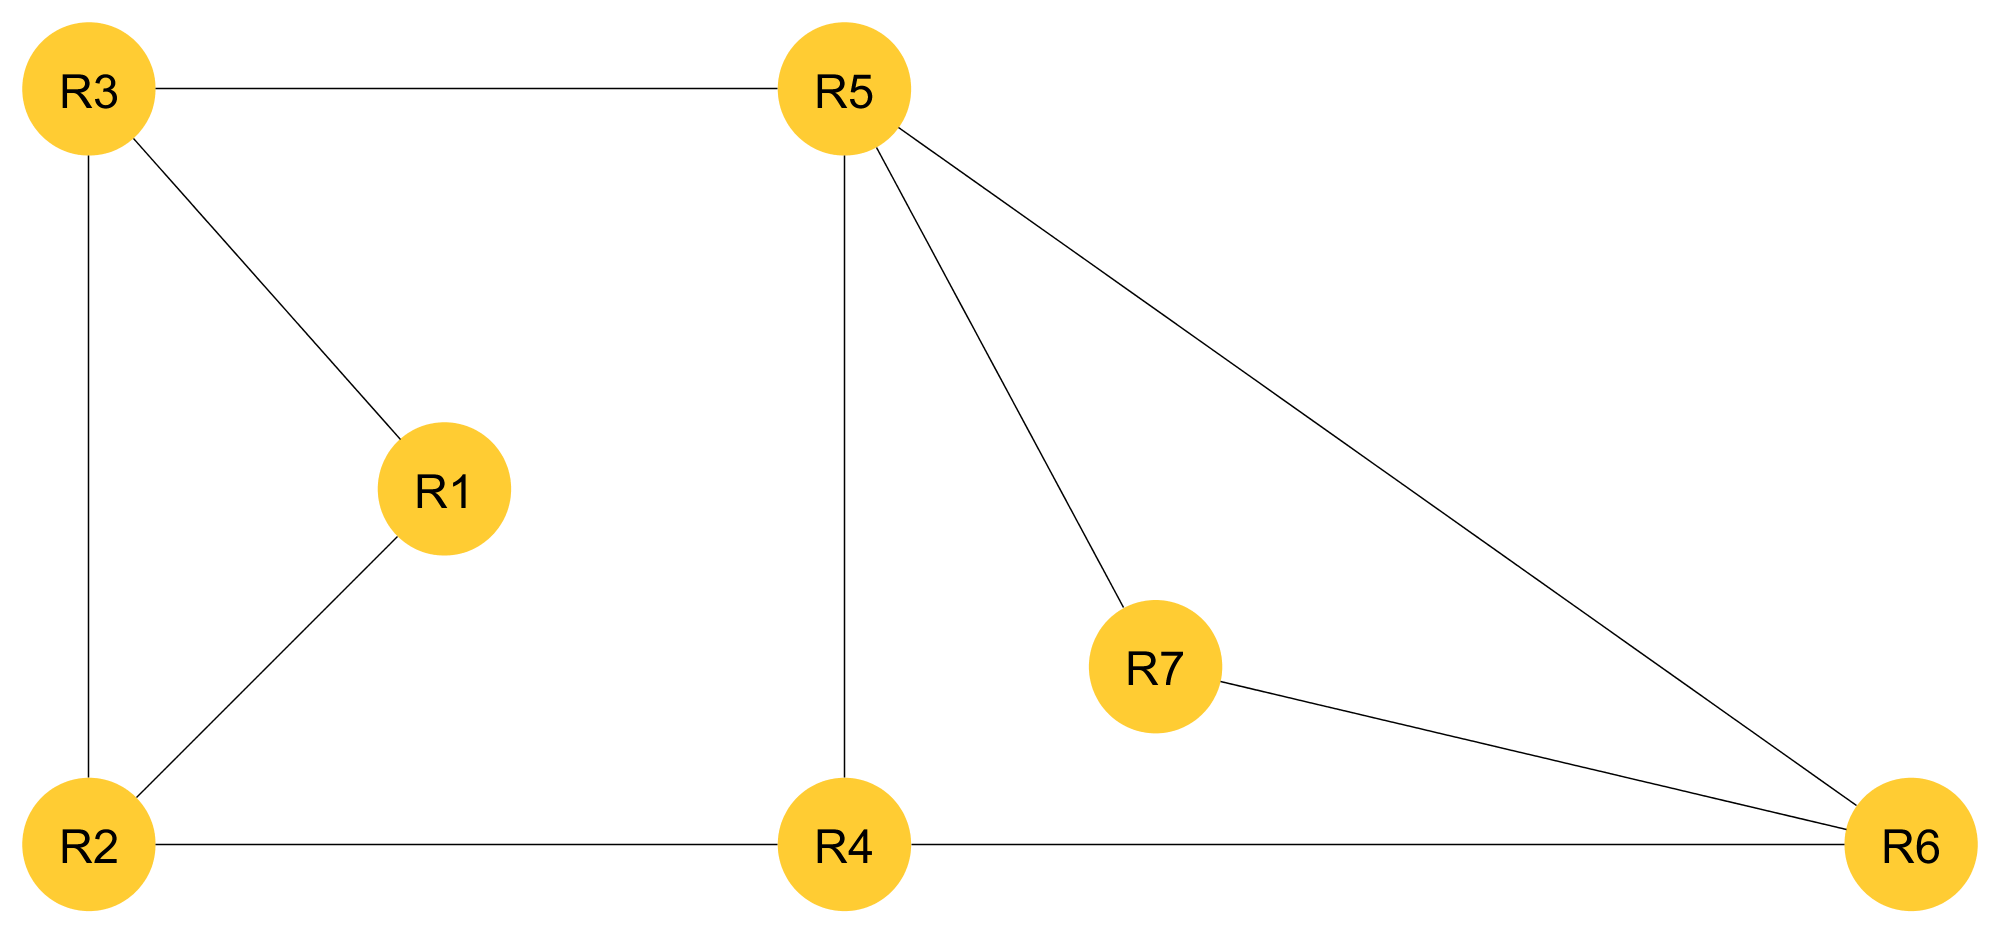
\includegraphics[width=14cm]{img/rip}
\end{center}

\textbf{1.} Si les routeurs suivent le protocole RIP, quel est la route empruntée par un paquet acheminé de R1 vers R7 ? Justifier.

\textbf{2.} Les routeurs sont maintenant configurés suivant le protocole OSPF. Les débits des interconnexions sont reportés ci-dessous :
\begin{center}
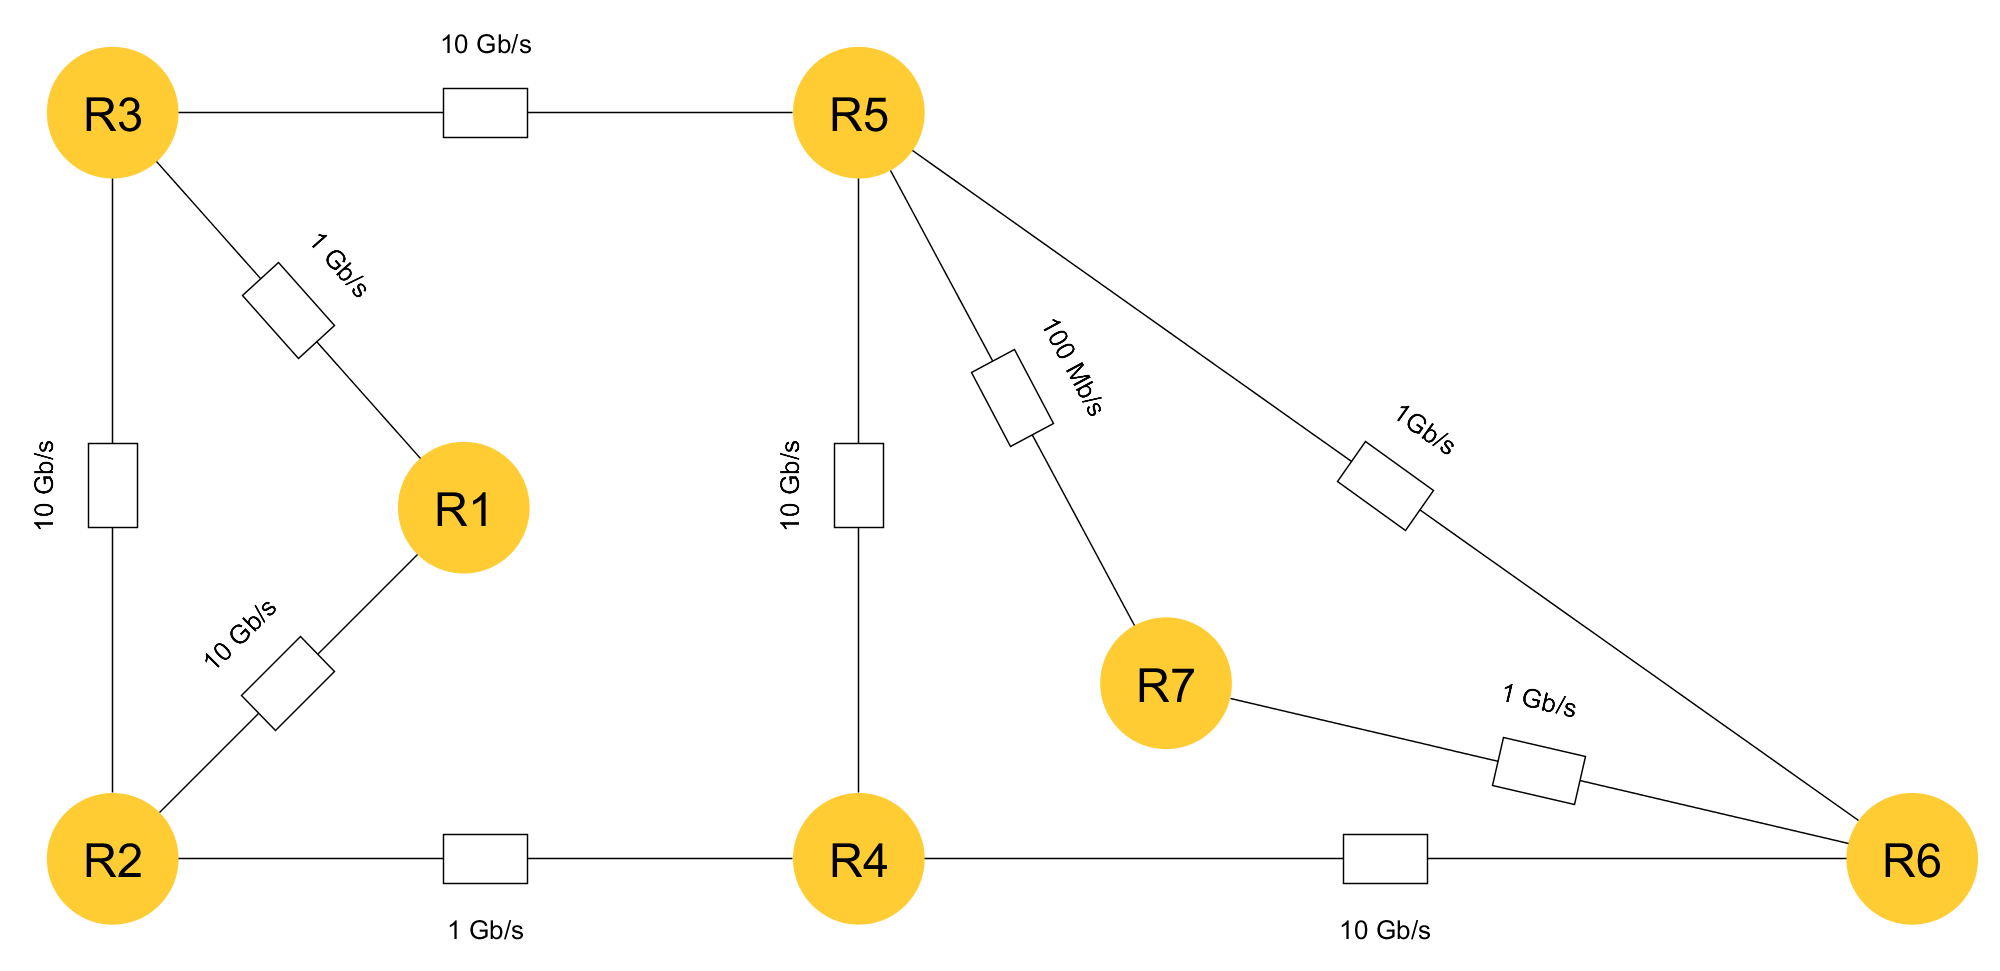
\includegraphics[width=14cm]{img/ospf}
\end{center}
\begin{enumerate}[\bfseries a.]
\item 	Reporter sur le graphe les coûts des connexions.
\item 	On veut connaître le chemin emprunté par un paquet transitant de R1 vers R7. Indiquer les coûts de chaque route et conclure.

\item Quel est le coût de la route choisie par le protocole RIP ?
\end{enumerate}
\end{exercice}
\end{document}